\documentclass[a4paper]{article}
\usepackage{blindtext}
\usepackage{csvsimple}
\usepackage{graphicx}
\usepackage{placeins}
\usepackage{hyperref}


\title{Project Phase 2}
\author{Baktash Ansari}
\date{\today}

\begin{document}  

\maketitle

GitHub repository  : \\

\href{https://github.com/baktash81/CS224nProject}{Repository}\\


\section{Introduction}

Before starting the explanations of different sections of Phase Two of the project, I would like to mention a few points:

\begin{enumerate}
  \item First and foremost, due to the large size of the imported models and the volume of training and testing parameters, most parts of this section (almost all of it) were executed remotely on Google Colab, and the results were saved locally. I tried to save as many parts as possible on my local machine (for example, parameters and loss values were saved), but the model and optimizer themselves were almost impossible to store due to their large size.
  \item All sections of the project, from Phase One to Phase Two, have been fully documented with comments and detailed explanations inside the notebook named "CrawDataNLProject" in the project directory on GitHub. You can review all my activities for this project in that notebook.
  \item The biggest challenge I faced during Phase Two was the hardware limitation. Specifically, I had a weak hardware setup, as I needed a GPU for the project, and the only GPU available to me was on Google Colab, which was also limited in terms of usage time (I had to switch between multiple accounts to avoid losing time).
\end{enumerate}

Ultimately, these challenges led me to work with a small portion of the dataset. For example, although I had around 300,000 to 600,000 sentences for each label, due to the limitations, I had to use only 10,000 to 15,000 of them.\\



To begin, I provide an explanation of the tasks I performed for each section, followed by presenting the results for better visibility.\\

\section{Word2Vec}


In this section, I used the gensim library to build and train my own word2vec model in order to create embeddings for the desired words. I utilized the skip-gram architecture and trained the model for 5 epochs. For the loss function, I used negative log likelihood.

Next, I selected a list of words and performed various analyses on them, which I will discuss in detail later.

\subsection*{Visualize word embeddings for each label}

In this section, I needed to visualize the words in a two-dimensional space. To achieve this, I had to reduce the dimensions using the \textbf{t-SNE}  algorithm. After dimensionality reduction of the word vectors, I used the \textbf{k-means}  algorithm to cluster the words into different groups, allowing us to observe their categorization.


The words I used in this section are as follows:\\

'fuck', 'stupid', 'nigga', 'girl', 'boy', 'toys', 'england', 'china', 'america', 'ghost',
      'car', 'horror', 'pink', 'black', 'red', 'asshole', 'love', 'heart', 'kiss', 'hug', 'pants',
      'shoes', 'hurt', 'suicide', 'hospital', 'gun', 'kill', 'police', 'doctor', 'arm', 'eye', 'leg',
      'house', 'park', 'cinema', 'office', 'canada', 'iran', 'korea'\\


I visualized these words separately for each label, and you can see the results for each label below.


\begin{figure}[ht]
    \centering
    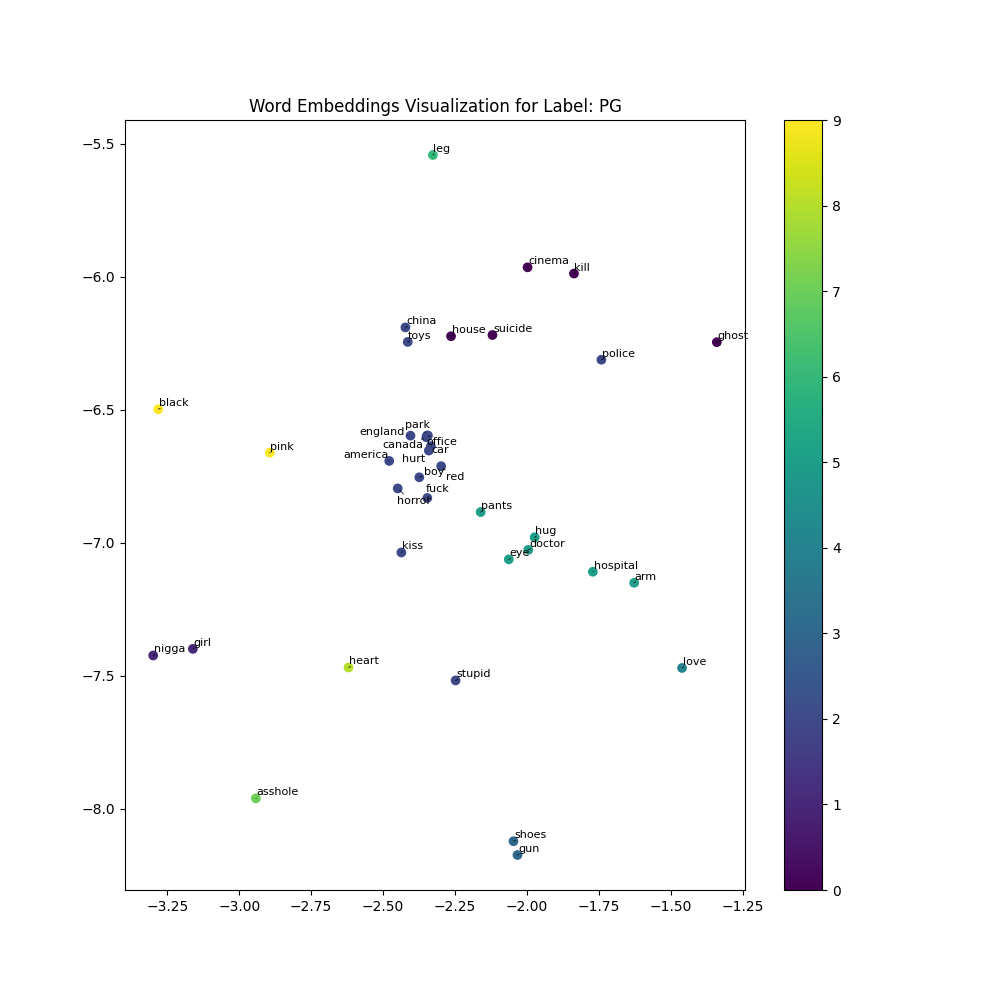
\includegraphics[width=1\textwidth]{../stats/word_embeddings_PG.png}
    \caption{Visualization}
\end{figure}

\begin{figure}[ht]
    \centering
    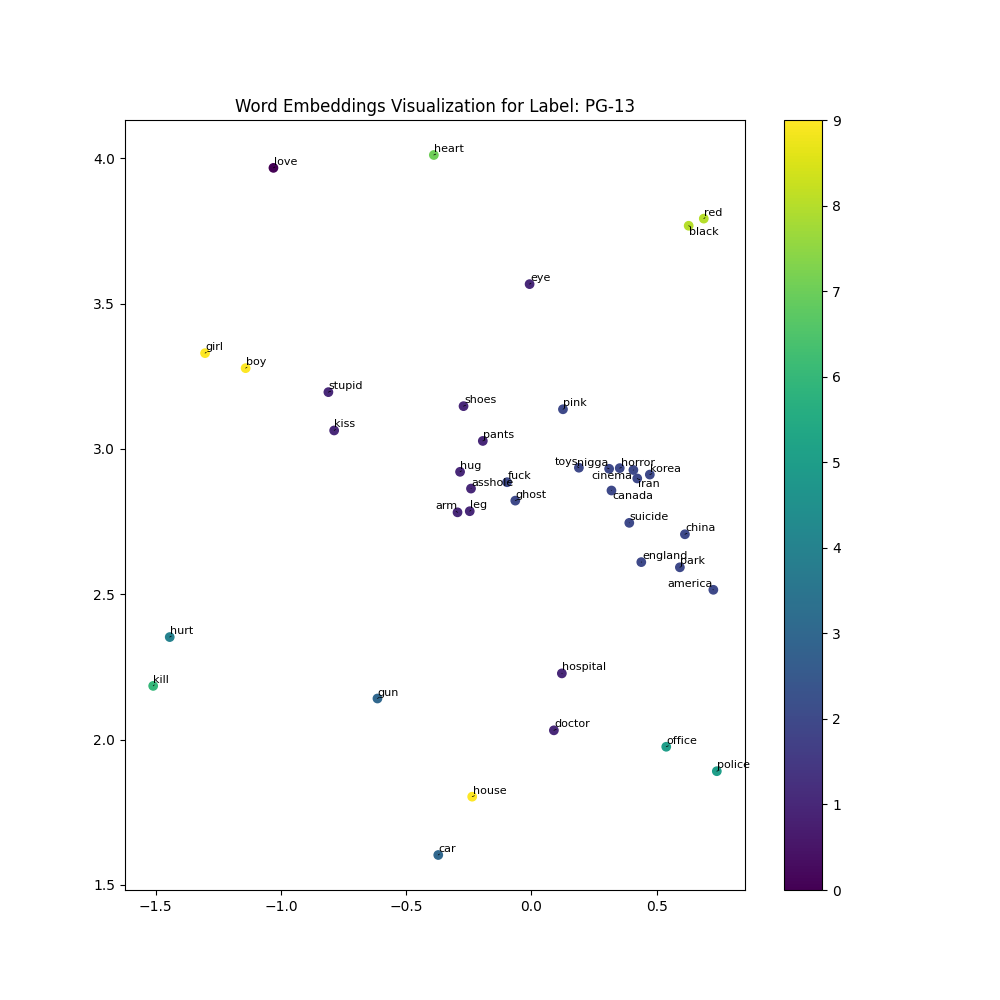
\includegraphics[width=1\textwidth]{../stats/word_embeddings_PG-13.png}
    \caption{Visualization}
\end{figure}

\begin{figure}[ht]
    \centering
    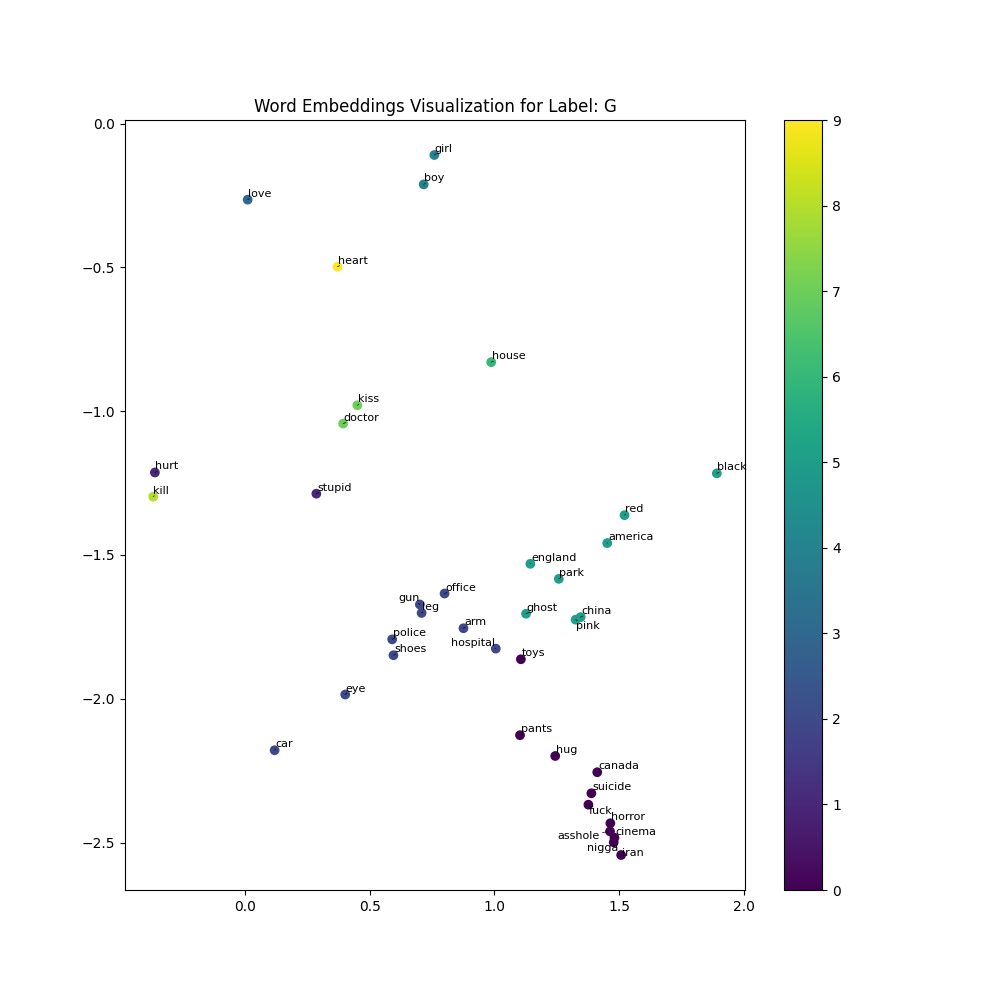
\includegraphics[width=1\textwidth]{../stats/word_embeddings_G.png}
    \caption{Visualization}
\end{figure}

\begin{figure}[ht]
    \centering
    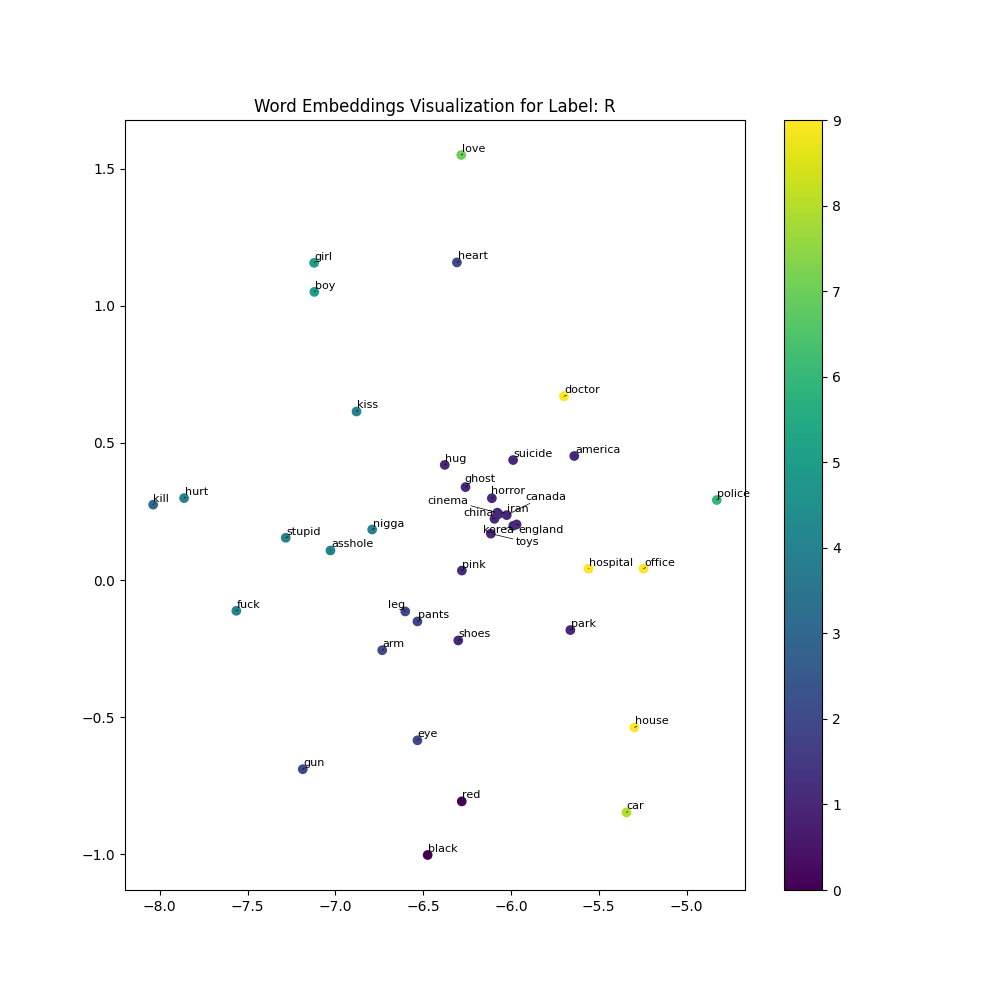
\includegraphics[width=1\textwidth]{../stats/word_embeddings_R.png}
    \caption{Visualization}
\end{figure}

\begin{figure}[ht]
    \centering
    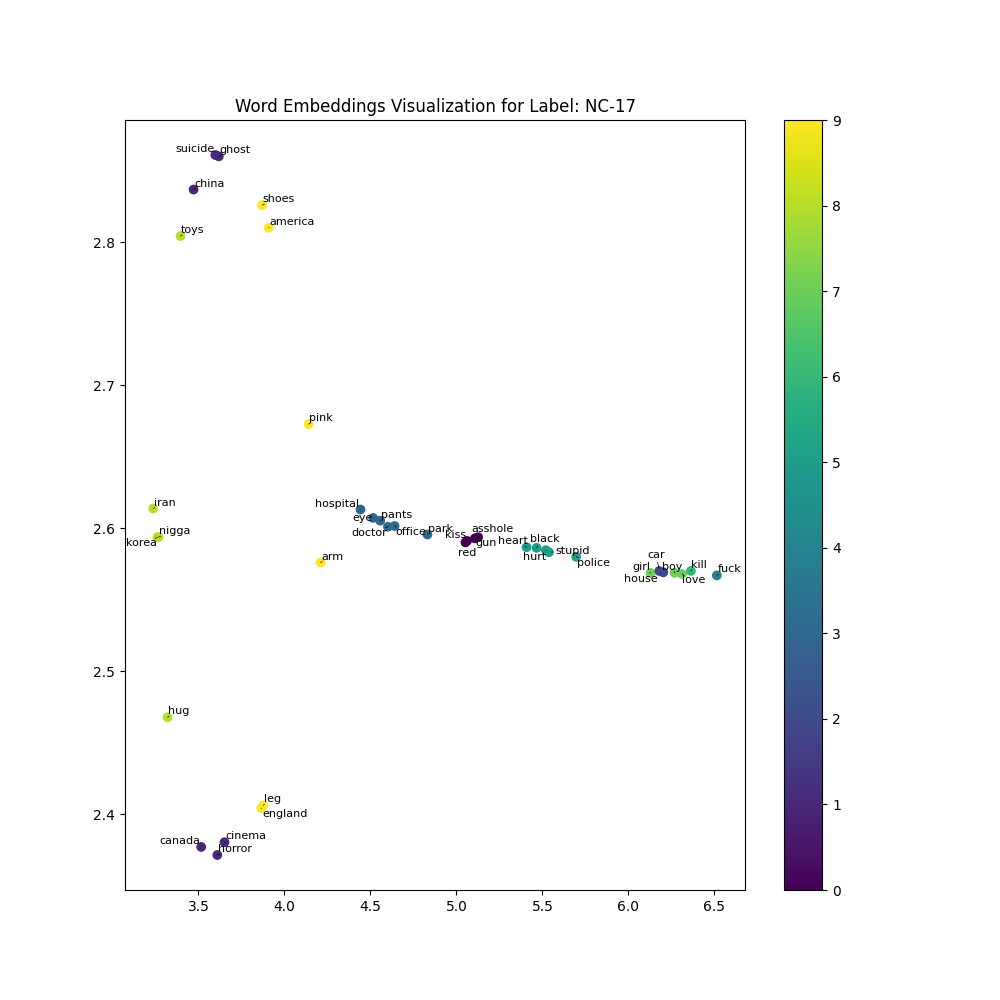
\includegraphics[width=1\textwidth]{../stats/word_embeddings_NC-17.png}
    \caption{Visualization}
\end{figure}

\FloatBarrier

\subsection*{Euclidean distance and cosine similarity of 20 common words between each pair of labels.}

Here, I calculated the distances between each pair of words from the previous words using these two metrics, and I stored them in a table called "Heatmap." I performed this process for each pair of labels. The generated plots can be seen after the description of the heatmap.

\subsection*{Heatmap}
A heatmap is a graphical representation of data in a matrix format, where different colors are used to indicate the magnitude of values. In the context of cosine similarity, a heatmap provides a visual representation of the similarity between pairs of words based on their word embeddings.

In the heatmap, each cell represents the similarity score between a pair of words. The similarity scores are calculated using the cosine similarity measure, which quantifies the similarity between two vectors by measuring the cosine of the angle between them.\\\\

\begin{figure}[ht]
    \centering
    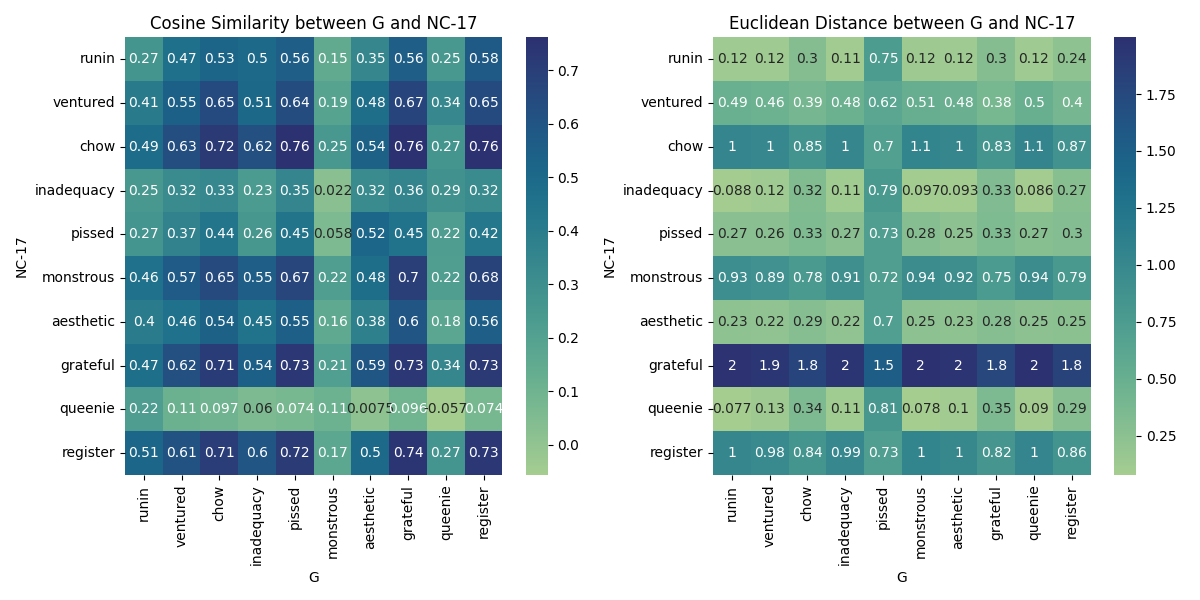
\includegraphics[width=1\textwidth]{../stats/HeatMap_G_NC-17.png}
    \caption{Heatmap}
\end{figure}

\begin{figure}[ht]
    \centering
    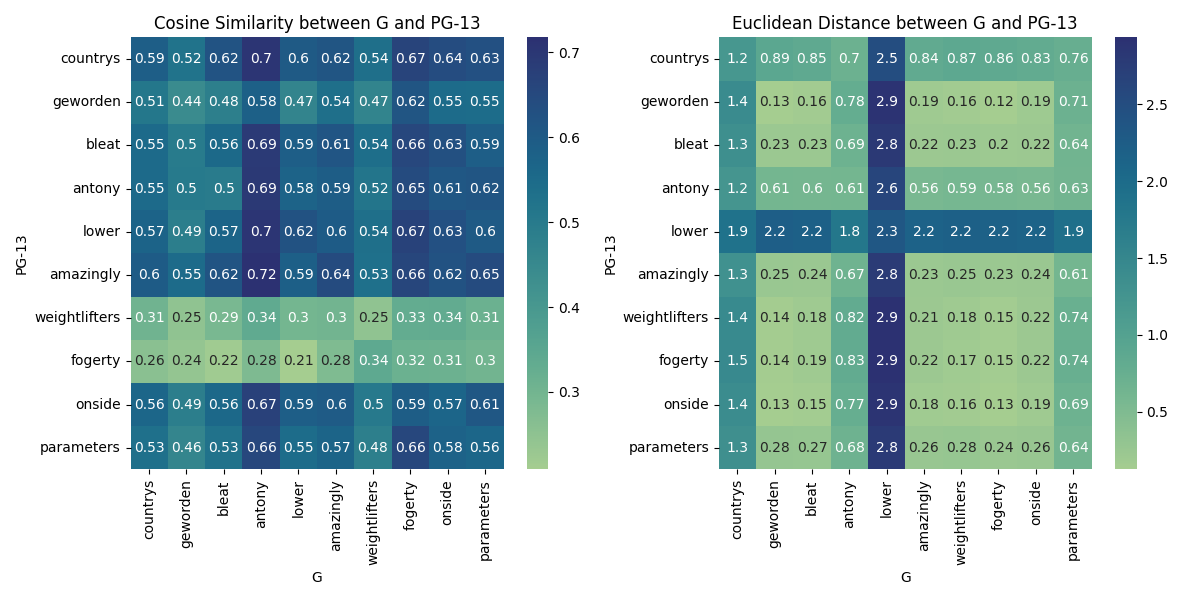
\includegraphics[width=1\textwidth]{../stats/HeatMap_G_PG-13.png}
    \caption{Heatmap}
\end{figure}

\begin{figure}[ht]
    \centering
    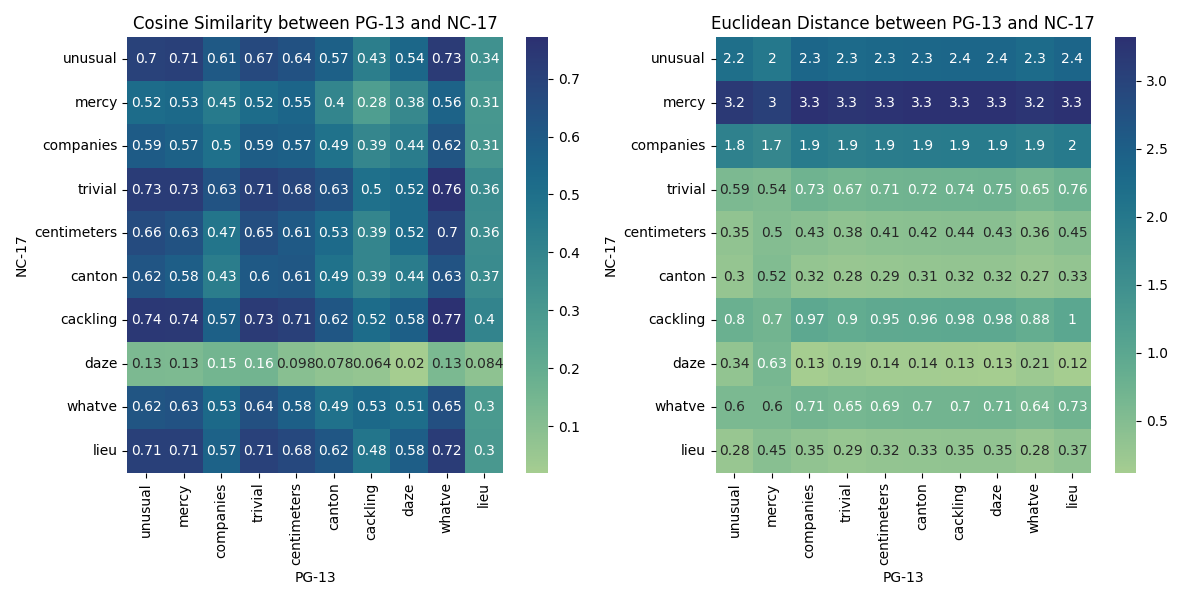
\includegraphics[width=1\textwidth]{../stats/HeatMap_PG-13_NC-17.png}
    \caption{Heatmap}
\end{figure}

\begin{figure}[ht]
    \centering
    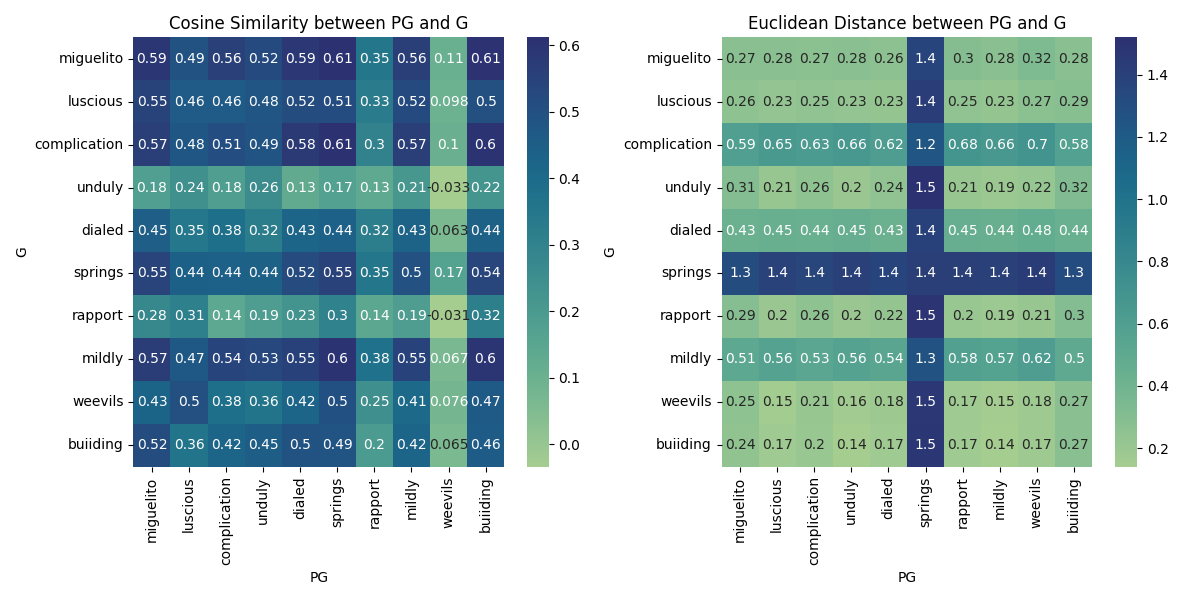
\includegraphics[width=1\textwidth]{../stats/HeatMap_PG_G.png}
    \caption{Heatmap}
\end{figure}

\begin{figure}[ht]
    \centering
    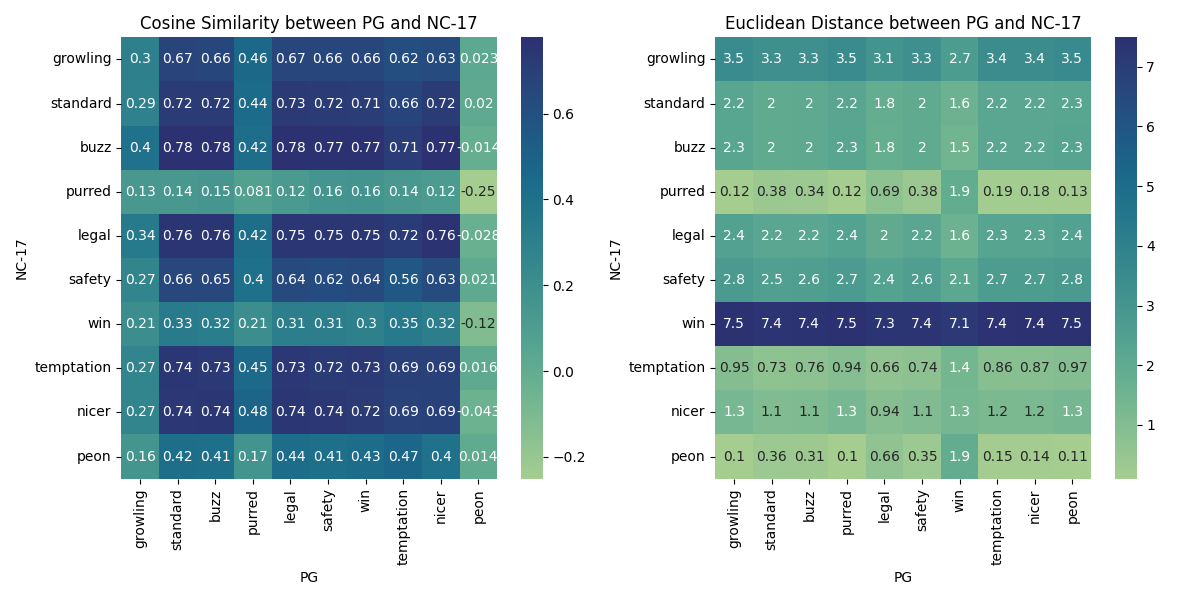
\includegraphics[width=1\textwidth]{../stats/HeatMap_PG_NC-17.png}
    \caption{Heatmap}
\end{figure}

\begin{figure}[ht]
    \centering
    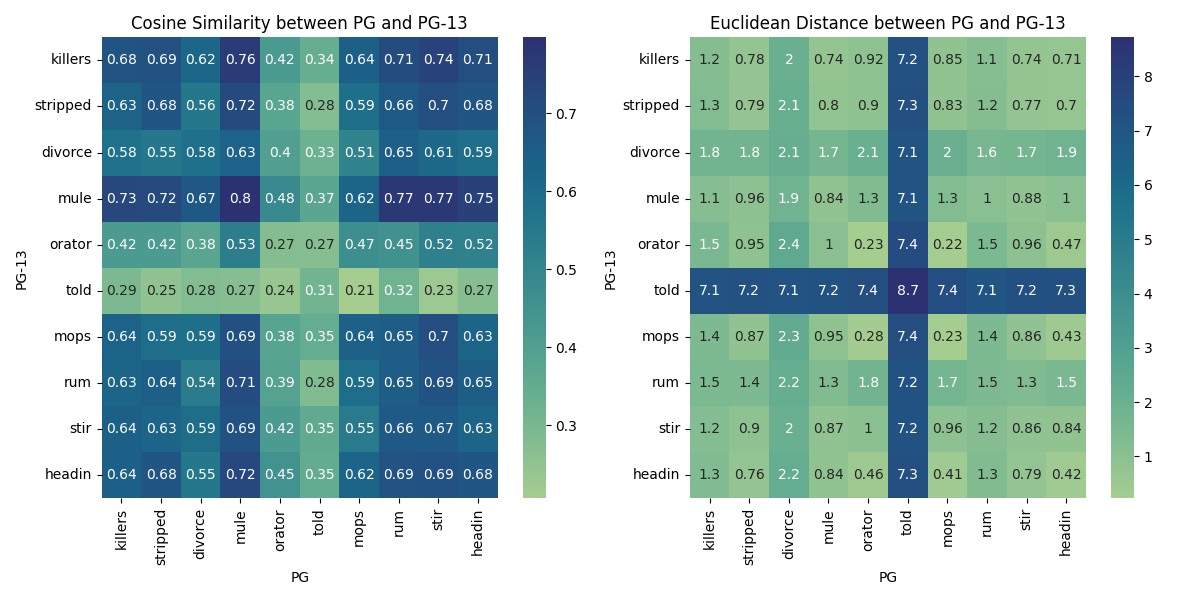
\includegraphics[width=1\textwidth]{../stats/HeatMap_PG_PG-13.png}
    \caption{Heatmap}
\end{figure}

\begin{figure}[ht]
    \centering
    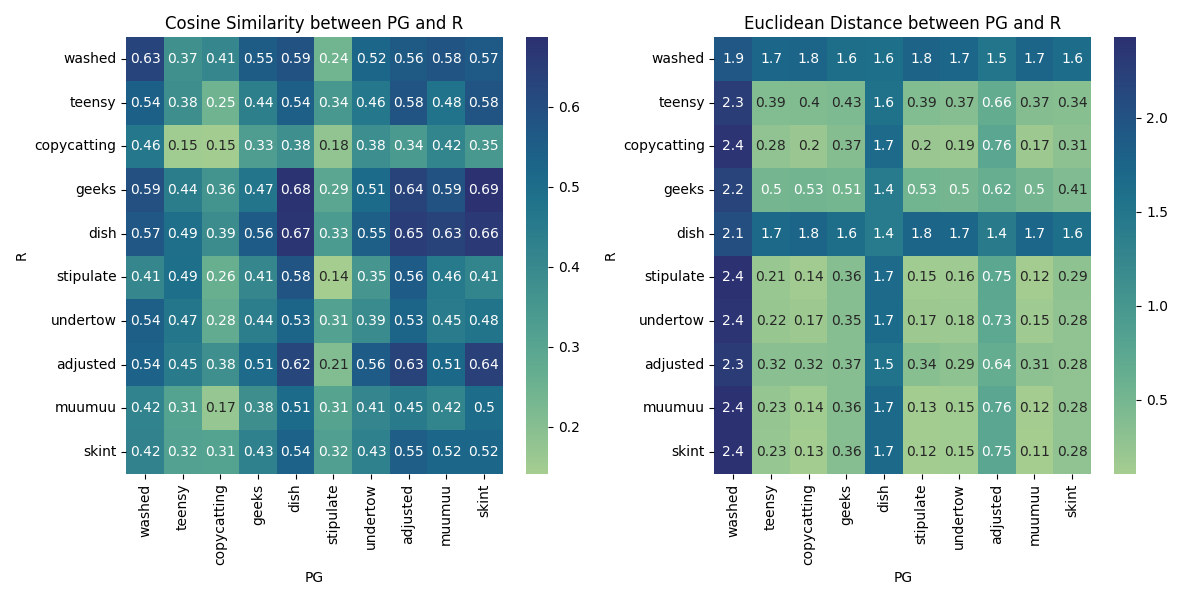
\includegraphics[width=1\textwidth]{../stats/HeatMap_PG_R.png}
    \caption{Heatmap}
\end{figure}

\begin{figure}[ht]
    \centering
    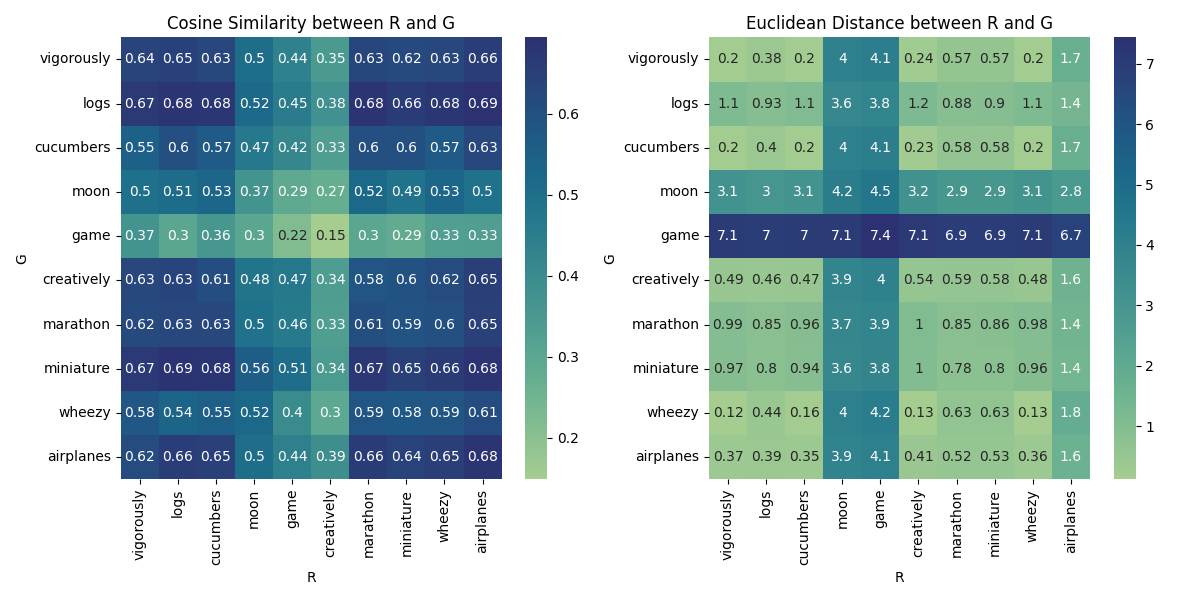
\includegraphics[width=1\textwidth]{../stats/HeatMap_R_G.png}
    \caption{Heatmap}
\end{figure}

\begin{figure}[ht]
    \centering
    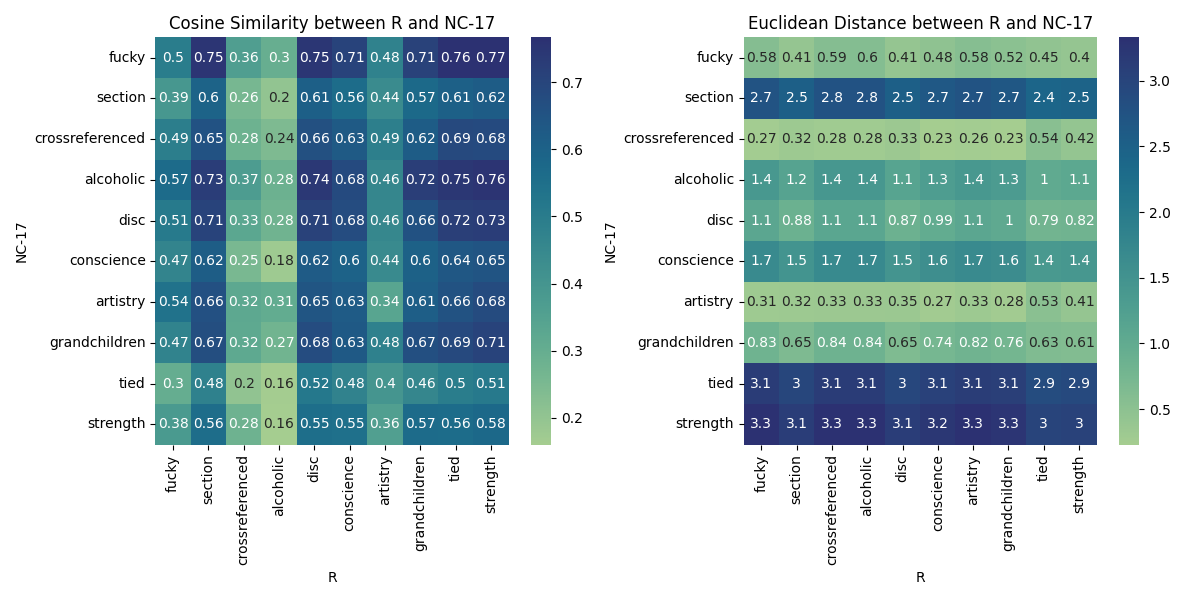
\includegraphics[width=1\textwidth]{../stats/HeatMap_R_NC-17.png}
    \caption{Heatmap}
\end{figure}

\begin{figure}[ht]
    \centering
    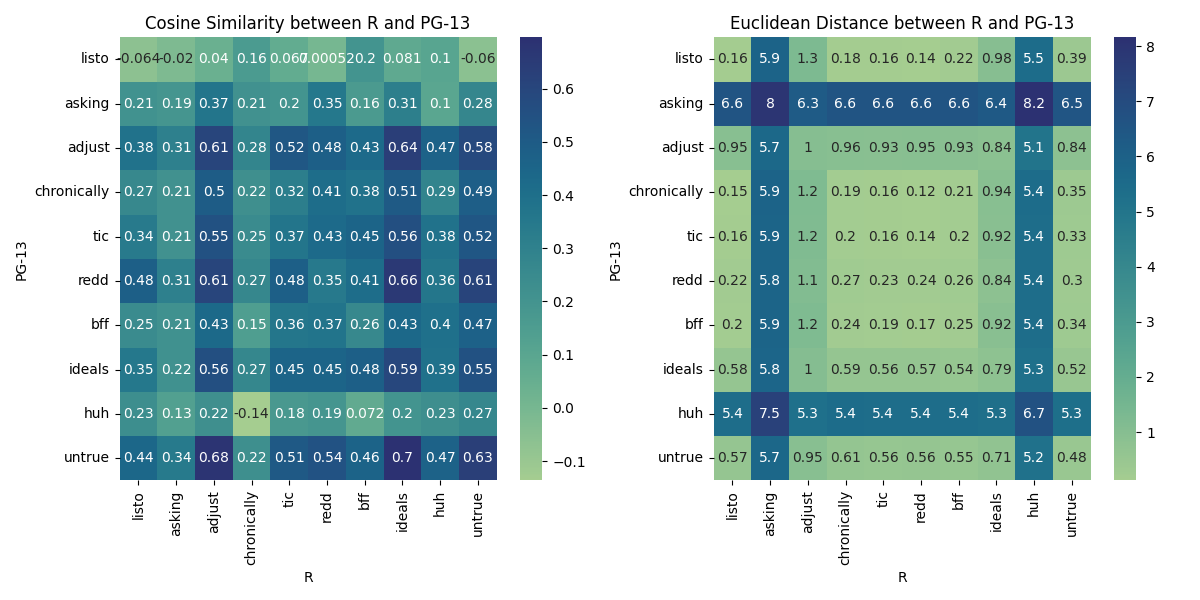
\includegraphics[width=1\textwidth]{../stats/HeatMap_R_PG-13.png}
    \caption{Heatmap}
\end{figure}

\FloatBarrier

For the word2vec section, I trained the models separately for each label and performed one round of training for all the words together. The created models can be found in the "models" directory and are visible for inspection.\\

At the end of this section, Cosine similarity to find top nearest words for specific word, for example for word \textbf{"america"} the result is : \\

\begin{center}
china 0.7783911228179932\\
europe 0.7576916217803955\\
france 0.7552369236946106\\
russia 0.7530403733253479\\
country 0.7460766434669495\\
england 0.7440224289894104\\
africa 0.7169732451438904\\
australia 0.677288293838501\\
germany 0.675476610660553\\
nation 0.6725935339927673\\
\end{center}

\section{Tokenization}

In this section,i used SentencePiece library for tokenization. in order to determine an appropriate vocabulary size, I selected a set of vocab sizes as follows:

\begin{center}
    500, 1000, 2000, 4000, 8000, 10000, 12500
\end{center}

I divided the data for each label into 5 parts, and training was conducted in 5 stages, with each stage consisting of 4 parts, while evaluation was performed on the remaining part. The evaluation process is expressed as the percentage of the "unk" token in the total tokens, which is displayed in a table below.\\

\begin{table}[ht]
    \centering
    \csvautotabular{../stats/tokenization_report_G.csv}
    \caption{Tokenization for label G}
    \label{tab:data}
\end{table}

\begin{table}[ht]
    \centering
    \csvautotabular{../stats/tokenization_report_NC-17.csv}
    \caption{Tokenization for label NC-17}
    \label{tab:data}
\end{table}

\begin{table}[ht]
    \centering
    \csvautotabular{../stats/tokenization_report_PG-13.csv}
    \caption{Tokenization for label PG-13}
    \label{tab:data}
\end{table}

\begin{table}[ht]
    \centering
    \csvautotabular{../stats/tokenization_report_R.csv}
    \caption{Tokenization for label R}
    \label{tab:data}
\end{table}

\begin{table}[ht]
    \centering
    \csvautotabular{../stats/tokenization_report_PG.csv}
    \caption{Tokenization for label PG}
    \label{tab:data}
\end{table}

\begin{table}[ht]
    \centering
    \csvautotabular{../stats/tokenization_report_All.csv}
    \caption{Tokenization for all labels together}
    \label{tab:data}
\end{table}

\FloatBarrier

As observed, the vocabulary size of 500 has significantly fewer "unk" tokens compared to the other sizes.

\section{Language model for text generating}

For this section, I used the GPT-2 model and utilized the available notebook on Kaggle (\href{https://www.kaggle.com/code/nulldata/fine-tuning-gpt-2-to-generate-netlfix-descriptions}{this notebook}). One of the major challenges I encountered in this section was the lack of suitable hardware and graphics capabilities. This made the task difficult to the extent that I had to downsize the data. I had to reduce the number of sentences for each label to 15,000 sentences. Even this number was quite challenging due to usage limitations and required approximately 1 hour per label.

Additionally, I couldn't save the models due to limitations in Google Drive space, so I had to save only the checkpoints every 5000 steps.

Despite all the difficulties in this section, I managed to generate sentences with a highly limited model, which, as you may guess, did not yield satisfactory results. However, you can still observe logical changes in the sentences within the labels, although the expectations were much higher than these values.

You can view the results.

\subsection*{PG}

\begin{center}
    0:  inaas well really see get way\\
1:  ive thought ever would think\\
2:   ay\\
3:  ive seen come live together much since arrival home day\\
4:  ian hes trying get us good night good night come ill work next\\
5:  ive put foot right far time last time want talk\\
6:  ibal yes l\\
7:  ive ever thought life looked pretty nice enough never\\
8:  ive got five nights keep away\\
9:  ichael youve got place mr roster\\
10:  ike always trying put little pressure\\
11:  ive never seen much\\
12:  ive really seen since first two hours\\
13:  ive found one moment courage keep taking care right right back lets leave tonight sleep\\
14:  ia heh\\
15:  ive actually got chance\\
16:  ies see\\
17:  ive since seen\\
18:  ina right right youre one okay\\
19:  ive taken a great step toward understanding new ways\\
\end{center}

\subsection*{PG-13}

\begin{center}
    0:  inaas well see see another way\\
    3:  yes come mr mama said\\
    4:  ive got trouble\\
    5:  ive put foot right feet today huh\\
    6:  leo tred leonnef oar\\
    7:  ive ever thought\\
    8:  izzies oh wow jingles\\
    9:  iam going kill us\\
    10:  iz coming thats coming\\
    11:  ive run\\
    12:  izzy yeah know cant remember name yet yet go get new one next call youve got come back like youve got\\
    13:  ive done little business right years\\
    14:  ive gone past\\
    15:  ive lost family yet\\
    16:  ik er\\
    17:  ive always want\\
    18:  ids find right thing one one something\\
    19:  icky shit\\
\end{center}

\subsection*{G}

\begin{center}
    0:  irmas well oh see another way\\
    1:  ive thought nothing except waiting today one last song oh uh ive done\\
    2:  ive loved music since\\
    3:  ive seen come live today today right tell us\\
    4:  ive picked around\\
    5:  ive put us right end house last time\\
    7:  ive ever thought life fun thought nice enough never\\
    8:  ive got go work late\\
    9:  ive watched little kids growing ever\\
    10:  ive always heard isnt mean\\
    11:  ive grown used much use love\\
    12:  ive really seen someone around town come out astrunk feet water away\\
    13:  ive found one back right side\\
    14:  ive gone crazy hell never seen\\
    15:  ive never saw yet\\
    16:  ik er\\
    17:  ive always seen\\
    18:  ive had idea youd nice nice try\\
    19:  icky must feel great pain\\
\end{center}

\subsection*{NC-17}

\begin{center}
    0:  ina need help oh okay sorry\\
    1:  ive thought nothing would happen today one way\\
    2:    sodging\\
    3:  ive seen come today today today right tell\\
    4:  ive forgotten\\
    5:  ive put foot right feet three feet would want\\
    6:  ivan\\
    7:  ive ever thought\\
    8:  ive gotten little mail jean\\
    9:  ichael say could see\\
    10:  ive always heard voice\\
    11:  ive never seen anyone get depressed\\
    12:  ive going\\
    13:  ive kept busy well enjoy good night today right right around huh\\
    14:  ive gone crazy hell around things right\\
    15:  ive never experienced yet\\
    16:  ive come away id want leave\\
    17:  ivan didnt want\\
    18:  ivan right right youlemnys\\
    19:  ive wanted watch watch\\
\end{center}

\subsection*{R}

\begin{center}
    0:  ive taken apart entire world since life\\
    1:  ive thought ever would move\\
    2:  ive already come talk\\
    3:  imeis come mmmm okay right\\
    4:  ive got money\\
    5:  ive put body right far house town would want know happened\\
    6:  ichris stowman dont come get phone back day ill wait\\
    7:  ive ever thought life life life may be like\\
    8:  ive gotten little hangover therestha waiting waiter im going go\\
    9:  ichael wenter\\
    10:  iev gon na put\\
    11:  ive never used much use car\\
    12:  ive slept little time alone know l am always dreaming im sleeping next hour\\
    13:  ive kept eye well seen lately\\
    14:  icky\\
    15:  ive told family yeta theyll never think\\
    16:  ies one\\
    17:  ive since seen\\
    18:  ickie right youre one girl\\
    19:  icky shit\\
\end{center}

\section{Classification model}

For the classification section, I used the BERT model available in the Hugging Face library. In this section, I first prepared the available data that I created in Phase One of the project with the corresponding labels (the complete code is available in the notebook). However, I had to use a small portion of the data for this section as well (20,000 records per label).

Then, I divided the data into train and test sets using the sklearn library and started the training process (with a ratio of 85\% for training and 15\% for testing). I manually conducted the training process, performing 5 epochs with a batch size of 16.

After each epoch, the models were saved in the "models" directory, and the log of each epoch was also stored in the "logs" folder.

For the evaluation section, I used metrics such as F1 score and accuracy per class, which can be seen in a table for each epoch.

\begin{table}[ht]
    \centering
    \csvautotabular{../stats/BERT_result.csv}
    \caption{BERT result}
    \label{tab:data}
\end{table}

\FloatBarrier

For class based evaluation we have : 

\begin{table}[ht]
    \centering
    \csvautotabular{../stats/BERT_result_class_based.csv}
    \caption{BERT result}
    \label{tab:data}
\end{table}

\FloatBarrier

For this section, I took assistance from the following link: \href{https://towardsdatascience.com/multi-class-text-classification-with-deep-learning-using-bert-b59ca2f5c613}{Link}.


\section{Fine tuning on chat-GPT API}

For this section, I created the desired data in the input format for the API and used the required API key. However, it seems that there are limitations on free APIs that do not allow the fine-tuning process. Nevertheless, the prompts and the related data for it are available in the GPT folder.\\\\

\section*{References}

For the resources, I utilized the documentation of the gensim and sentencepiece libraries, as well as the links I mentioned earlier. I also relied on my dear friend, ChatGPT, for assistance.

\end{document}